% ================================================================
% PART 2 — ATURAN PENULISAN JURNAL UNIVERSITAS BANI SALEH FTID
% ================================================================
\newpage

\begin{center}
    {\large\bfseries ATURAN PENULISAN JURNAL UNIVERSITAS BANI SALEH FTID\par}
\end{center}

\vspace{4pt}
\normalsize

\section{JUDUL}
Judul utama (pada halaman pertama) harus dituliskan dengan jarak margin 3
cm dari tepi kertas, rata tengah dan dalam huruf kapital Times New Roman 14, tebal.

\section{PENULIS DAN INSTITUSI}
Nama Penulis dan asal institusi (afiliasi) dituliskan dengan Times New Roman
12, spasi 1, Bold dengan jarak margin 3 cm dari tepi kertas, rata tengah.

\section{ABSTRAK}
Abstrak ditulis menggunakan Times New Roman 11, spasi 1, dan ditulis
maksimal 250 kata. Abstrak memuat uraian singkat mengenai masalah dan tujuan
penelitian, metode yang digunakan, dan hasil penelitian. Tekanan penulisan abstrak
terutama pada hasil penelitian. Abstrak ditulis dalam bahasa Indonesia dan Bahasa
Inggris. Kata kunci perlu dicantumkan untuk menggambarkan ranah masalah yang
diteliti dan istilah-istilah pokok yang mendasari pelaksanaan penelitian. Kata-kata kunci
dapat berupa kata tunggal atau gabungan kata. Jumlah kata-kata maksimal 5 kata.
Kata-kata kunci ini diperlukan untuk komputerisasi. Pencarian judul penelitian dan
abstraknya dipermudah dengan kata-kata kunci tersebut.

\section{PENDAHULUAN}
Bagian pendahuluan terutama berisi: (1) permasalahan penelitian; (2) wawasan
dan rencana pemecahan masalah; (3) kajian teoritik yang berkaitan dengan masalah
yang diteliti (\textit{gap research}), (4) rumusan tujuan penelitian. Pada bagian ini kadang-
kadang juga dimuat harapan akan hasil dan manfaat penelitian. Panjang bagian
pendahuluan sekitar 2-3 halaman dan diketik dengan 1 spasi Times New Roman 12.

\section{TINJAUAN PUSTAKA}
Teori yang mendukung variabel yang dibahas berdasarkan artikel sebelumnya
yang relevan, pengembangan hipotesis yang didasarkan atas teori dari penelitian
terdahulu (jika menggunakan hipotesis) dan kerangka pikir.

\section{METODE PENELITIAN}
Bagian ini menjelaskan bagaimana penelitian itu dilakukan. Materi pokok
bagian ini adalah: (1) rancangan penelitian; (2) populasi dan sampel (sasaran
penelitian); (3) teknik pengumpulan data dan pengembangan instrumen; (4) dan teknik
analisis data. Untuk penelitian yang menggunakan alat dan bahan, perlu dituliskan
spesifikasi alat dan bahannya. Spesifikasi alat menggambarkan kecanggihan alat yang
digunakan sedangkan spesifikasi bahan menggambarkan macam bahan yang digunakan.

Untuk penelitian kualitatif seperti penelitian tindakan kelas, etnografi,
fenomenologi, studi kasus, dan lain-lain, perlu ditambahkan kehadiran peneliti, subyek
penelitian, informan yang ikut membantu beserta cara-cara menggali data-data
penelitian, lokasi dan lama penelitian serta uraian mengenai pengecekan keabsahan hasil
penelitian. Sebaiknya dihindari penulisan ke dalam ``anak sub-judul'' pada bagian ini.

\section{HASIL DAN PEMBAHASAN}
Bagian ini merupakan bagian utama artikel hasil penelitian dan biasanya
merupakan bagian terpanjang dari suatu artikel. Hasil penelitian yang disajikan dalam
bagian ini adalah hasil ``bersih''. Proses analisis data seperti perhitungan statistik dan
proses pengujian hipotesis tidak perlu disajikan. Hanya hasil analisis dan hasil
pengujian hipotesis saja yang perlu dilaporkan. Tabel dan grafik dapat digunakan untuk
memperjelas penyajian hasil penelitian secara verbal. Tabel dan grafik harus diberi
komentar atau dibahas.

Untuk penelitian kualitatif, bagian hasil memuat bagian-bagian rinci dalam
bentuk sub topik-sub topik yang berkaitan langsung dengan fokus penelitian dan
kategori-kategori.

Pembahasan dalam artikel bertujuan untuk: (1) menjawab rumusan masalah dan
pertanyaan-pertanyaan penelitian; (2) menunjukkan bagaimana temuan-temuan itu
diperoleh; (3) menginterpretasi/menafsirkan temuan-temuan; (4) mengaitkan hasil
temuan penelitian dengan struktur pengetahuan yang telah mapan; dan (5)
memunculkan teori-teori baru atau modifikasi teori yang telah ada.

Dalam menjawab rumusan masalah dan pertanyaan-pertanyaan penelitian, hasil
penelitian harus disimpulkan secara eksplisit. Penafsiran terhadap temuan dilakukan
dengan menggunakan logika dan teori-teori yang ada. Temuan berupa kenyataan di
lapangan diintegrasikan/dikaitkan dengan hasil-hasil penelitian sebelumnya atau
dengan teori yang sudah ada. Untuk keperluan ini harus ada rujukan. Menjelaskan
implikasi teoritis dan implikasi praktis dari temuan penelitian.

\section{PENUTUP}
\subsection{Simpulan}
Simpulan menyajikan ringkasan dari uraian mengenai hasil dan pembahasan,
mengacu pada tujuan penelitian, bukan mengulang teori dan tidak berisi angka statistik,
dibuat tanpa sub judul. Berdasarkan kedua hal tersebut dikembangkan pokok-pokok
pikiran baru yang merupakan esensi dari temuan penelitian.

\subsection{Saran}
Saran disusun berdasarkan temuan penelitian yang telah dibahas. Saran dapat
mengacu pada tindakan praktis, pengembangan teori baru, dan/atau penelitian lanjutan.

\section{REFERENSI}
\noindent Penulisan referensi menggunakan sistem MENDELEY (gunakan \textit{reference manager}).
Tidak perlu dikelompokkan berdasarkan buku, jurnal, koran, ataupun berdasarkan tipe
publikasi lainnya.

\vspace{4pt}
\noindent Tulisan atau naskah adalah asli, belum pernah diterbitkan/dipublikasikan di media
cetak lain. Naskah adalah hasil karya penulis berupa riset lapangan maupun riset kepustakaan
yang mengkaji permasalahan aktual yang berkembang di masyarakat.

\vspace{4pt}
\noindent Tulisan ilmiah menggunakan bahasa Indonesia baku, setiap kata asing dicari
padanannya dalam bahasa Indonesia baku, dan tidak perlu menyertakan bahasa
asingnya. Kalimat yang diambil dari tulisan ilmiah dalam bahasa asing diterjemahkan dalam
bahasa Indonesia baku.

\vspace{4pt}
\noindent Referensi menggunakan aturan MENDELEY dengan APA \textit{style} dan tidak
menggunakan catatan kaki.

\vspace{12pt}
\noindent\colorbox{yellow!70}{\parbox{\dimexpr\linewidth-2\fboxsep}{Tulisan ilmiah dikirimkan dengan format:}}

\begin{itemize}[leftmargin=1.6cm]
    \item Naskah diketik dalam 1 (satu) spasi dengan menggunakan Ms. Word (Font
          Times New Roman, ukuran 12 pitch), dengan jumlah kata minimal 3500--5500
          kata atau 8--15 halaman kertas A4 (sudah termasuk gambar, tabel, ilustrasi,
          dan daftar pustaka), dengan batas pengetikan adalah batas kiri, batas kanan,
          batas atas dan batas bawah = 3 cm.
    \item Naskah dibuat dalam bentuk 1 kolom (standar).
    \item Semua jenis rumus ditulis menggunakan \textit{Mathematical Equation} (bagi
          pengguna MS Word ada di bagian Insert => Equation), termasuk
          pembagian/fraksi, Sigma, Akar, Matriks, Integral, Limit/Log, Pangkat, dsb.
\end{itemize}

\vspace{10pt}
\subsection{Gambar dan Tabel}
\noindent Tempatkan label tabel di atas tabel, sedangkan label gambar di bagian bawah gambar. Font
Times New Roman, ukuran 10 pitch. Tuliskan tabel tertentu secara spesifik, misalnya
Tabel 1, saat merujuk suatu tabel. Contoh penulisan tabel dan keterangan gambar adalah
sebagai berikut:

\begin{center}
    \footnotesize
    \textbf{Tabel 1.} Format Tabel\\[4pt]
    \renewcommand{\arraystretch}{1.3}
    \begin{tabular}{p{2.4cm}p{3.4cm}p{3.4cm}}
        \hline
        \textbf{Kepala Tabel} & \multicolumn{2}{c}{\textbf{Kepala Kolom Tabel}}                             \\
                              & \textbf{Sub-kepala Kolom}                       & \textbf{Sub-kepala Kolom} \\
        \hline
        Isi                   & Isi tabel                                       & Isi tabel                 \\
        \hline
    \end{tabular}
\end{center}

\vspace{10pt}
\begin{center}
    % --- example figure recreated as a vector diagram ---
    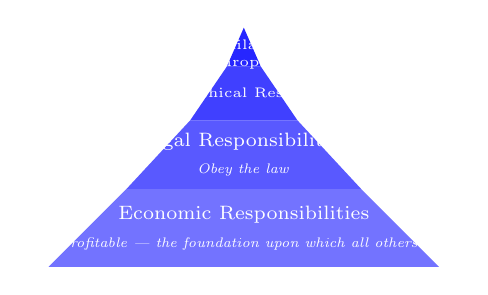
\begin{tikzpicture}[scale=0.62, every node/.style={font=\scriptsize, align=center, text=white}]
        \def\layers{{"Ethical\\Responsibilities","Legal\\Responsibilities","Economic\\Responsibilities"}}
        % base (economic)
        \fill[blue!55] (0,0) -- (8,0) -- (6.4,1.6) -- (1.6,1.6) -- cycle;
        \node at (4,0.8) {Economic Responsibilities\\[2pt]\tiny\textit{Be profitable — the foundation upon which all others rest}};
        % legal
        \fill[blue!65] (1.6,1.6) -- (6.4,1.6) -- (5.1,3.0) -- (2.9,3.0) -- cycle;
        \node at (4,2.3) {Legal Responsibilities\\[2pt]\tiny\textit{Obey the law}};
        % ethical
        \fill[blue!75] (2.9,3.0) -- (5.1,3.0) -- (4.35,4.1) -- (3.65,4.1) -- cycle;
        \node at (4,3.55) {\tiny Ethical Resp.};
        % philanthropic (apex)
        \fill[blue!85] (3.65,4.1) -- (4.35,4.1) -- (4,4.9) -- cycle;
        \node[font=\fontsize{5}{6}\selectfont] at (4,4.35) {Philan-\\thropic};
    \end{tikzpicture}
    \\[2pt]
    \textbf{Gambar 1.} \textit{Contoh Piramida Tanggung Jawab Sosial Perusahaan}
\end{center}

\subsection{Kutipan dan Acuan}
\noindent Penulis disarankan menggunakan fasilitas bantu sitasi, seperti Zotero, Endnote, atau
Mendeley untuk memastikan cara pengacuan dan penulisan daftar pustaka yang sesuai
dengan gaya penulisan di jurnal Tridi.

\begin{enumerate}[leftmargin=1.6cm,label=\alph*.]
    \item Sumber kutipan dalam teks ditulis di antara kurung buka dan kurung tutup yang
          menyebutkan nama belakang (akhir) penulis, tahun, dan nomor halaman. Contoh:
          \begin{enumerate}[leftmargin=1cm,label=\arabic*.]
              \item Satu sumber kutipan dengan satu penulis: (Asyik, 2006), jika disertai
                    dengan halaman: (Asyik, 2006: 289)
              \item Satu sumber kutipan dengan dua penulis: (Cooper dan Schlinder, 2003: 24)
              \item Satu sumber kutipan lebih dari dua penulis: (Guan et al., 2009)
          \end{enumerate}
    \item Jika penulis lebih dari dua orang, hanya nama penulis pertama yang disebutkan pada
          teks. Contoh: Guan et al. (2009: 59) menyatakan\ldots
    \item Dua sumber kutipan dengan penulis yang sama: John (2006, 2007); jika tahun
          publikasi sama: Sumiyana (2007a, 2007b).
    \item Sumber kutipan berupa banyak pustaka dengan penulis yang berbeda-beda:
          (Yermack, 1997; Aboody dan Kasznik, 2000; Guan et al., 2000).
    \item Sumber kutipan tidak menyebut nama penulis, tetapi menyebut suatu lembaga atau
          badan tertentu: Badan Pusat Statistik (2006).
    \item Apabila kutipan diambil dari sumber yang penulisnya mengutip dari sumber yang
          lain, maka ditulis seperti contoh: Simson, 1969 (dalam Aboody dan Kasznik,
          2000:321) menyatakan bahwa mayoritas perusahaan publik mengungkap pengaruh
          pro forma atas kompensasi berbasis saham di bawah pendekatan nilai wajar.
\end{enumerate}

\vspace{10pt}
\begin{center}
    \textbf{Contoh Penulisan referensi dengan APA \textit{style}}
\end{center}

% List ini tidak dihapus, hanya untuk mempertahankan wujud visual pada Panduan.
% Namun Daftar Pustaka ASLI pada dokumen kita sudah dibuat full OTOMATIS dan mengikuti indentasi yang sama seperti ini.
\begin{list}{}{\leftmargin=1.25cm \itemindent=-1.25cm \itemsep=8pt \small}

    \item Bank Indonesia Bandung. (2015). \textit{Statistik Ekonomi Keuangan Daerah bulan Pebruari}: Bandung.

    \item Dewinta, I. A., \& Setiawan, P. E. (2016). Pengaruh Ukuran Perusahaan, Umur
          Perusahaan, Profitabilitas, Leverage, Dan Pertumbuhan Penjualan Terhadap Tax
          Avoidance. \textit{E-Jurnal Akuntansi Universitas Udayana}, \textit{Vol.14.3. Maret}, 1584--1613.

    \item Febrianti, W. (2014). \textit{Pengaruh Kompensasi terhadap Etos Kerja dan Dampaknya
              terhadap Kinerja Karyawan pada PT. Artha Retailindo}. Skripsi. STIE
          Muhammadiyah: Jakarta. (Tidak dipublikasikan).

\end{list}